\documentclass[12pt,a4paper]{article}
\usepackage{a4wide}
\usepackage[english]{babel}
\usepackage[utf8]{inputenc}
\usepackage[alf]{abntex2cite}
\usepackage{amsmath}
\usepackage{enumitem}
\usepackage{geometry} 
\usepackage{graphicx}
\usepackage{float}

\title{
    {\small 
        Universidade de São Paulo\\
        Faculdade de Filosofia, Ciências e Letras de Ribeirão Preto\\
        Departamento de Computação e Matemática\\[1cm]
    }

    \vspace*{\fill}
    Comparing the LMC Complexity of Neural Networks with their Inference Capability
    \vspace*{\fill}
}
\author{
    Author: Lucas Miranda Mendonça Rezende\\ 
    Supervisor: Ph.D. Luiz Otavio Murta Junior
}
\date{\today}

\setlength{\parskip}{.5ex}

\begin{document}
    \pagenumbering{gobble}
        \maketitle

    \newpage
    \pagenumbering{arabic}
        \vspace*{\fill}
            \begin{abstract}
                TO DO
            \end{abstract}
        \vspace*{\fill}

    \newpage
        \tableofcontents

    \newpage
    \section{Introduction}

    Since the creation of Transformers and the Large Language Models (LLMs) based on this technique~\cite{vaswani2017attention}, there has been a veritable gold rush within the machine learning world. The exponential growth in AI investments and research has led to increasingly sophisticated models with remarkable capabilities~\cite{brown2020language, bubeck2023sparks}.

    However, over time, the need for more and more data to train increasingly larger models has become an impediment to the progress of these models' inference performance due to cost considerations~\cite{kaplan2020scaling, hoffmann2022training}. The scaling laws for neural language models demonstrate that performance improvements require exponentially increasing computational resources and training data, making further advancement increasingly expensive and resource-intensive.

    This creates the need for new advances that do not depend on adding more data but are instead improvements to the method itself, similar to what occurred with the creation of transformers~\cite{vaswani2017attention}. New methods to be created are generally based on observations of measures and relationships in the model weights.

    One such measure was investigated in recent research that explores the relationship between the well-known measure of model complexity and inference capability~\cite{murta2025complexity}. Understanding this relationship could provide insights into model efficiency and performance optimization without requiring massive increases in training data or computational resources.

    \subsection{Objective}

        \textbf{Work thesis}: There exists a relationship between model complexity and its inference capability~\cite{murta2025complexity}.

        The primary objectives of this work are to:
        \begin{itemize}
            \item Validate the hypothesis that model complexity and inference capability are related
            \item Measure and define the specific relationship that exists between these two measures, investigating whether complexity measures can serve as predictors of model performance across different architectures and tasks
        \end{itemize}

    \newpage
    \section{Methodology}

\subsection{Computational Environment}

\subsection{Model Selection}

Due to the wide availability of open models combined with the ease of accessing them through its Transformers library [https://arxiv.org/abs/1910.03771], \textbf{HuggingFace} was chosen as the source for model selection in this study.

HuggingFace is a platform that hosts a wide variety of machine learning models, datasets, and tools. It is widely used in the AI research community for sharing and collaborating on machine learning projects. [\url{https://www.researchgate.net/profile/Tejashree-Moharekar/publication/383497950_Hugging_Face_Revolutionizing_AI_and_NLP/links/66d036f8f84dd1716c702445/Hugging-Face-Revolutionizing-AI-and-NLP.pdf}] [https://huggingface.co/] Other platforms such as Ollama were considered, but ultimately not chosen due to the limited number of models and lack of company diversity. 

Model selection proceeded in two stages:

\begin{enumerate}
    \item First, we identified major technology companies by market capitalization that publish openly released language models. The companies considered were \textbf{OpenAI}, \textbf{Google}, \textbf{Meta} and \textbf{Microsoft}.
    \item Second, for each company we compiled a candidate set consisting of every model that satisfied the following criteria:
    
        \begin{itemize}
            \item Must be available on the HuggingFace platform.
            \item The model is a transformer-based language model.
            \item Model weights are publicly accessible (open weights), including models released behind
            gated access.
            \item The model is text-only (no multimodal image/audio inputs), .
            \item The model is an original base model rather than a task-specific fine-tuned variant.
            \item The total parameter count is below 150 billion. This upper bound was imposed due to
            hardware and inference limitations in the computational environment used for our experiments.
            \item The model is supported by the HuggingFace Transformers library [https://arxiv.org/abs/1910.03771] (i.e., it can be
            instantiated via the AutoModel/AutoTokenizer utilities), which ensures consistent loading and
            preprocessing across the candidate set.
            \item There's at least one publicly available benchmark result for the model among the selected benchmarks (section \ref{sec:benchmark_selection}).
        \end{itemize}

        The final selection of models used in this study is listed in Table \ref{tab:selected_models}.

        \begin{table}[H]
            \begin{tabular}{p{0.24\linewidth} p{0.24\linewidth} p{0.24\linewidth} p{0.24\linewidth}}
                \hline
                Meta & Google & Microsoft & OpenAI \\
                \hline
                meta-llama/Llama-4-Scout-17B-16E & google/gemma-3-27b-pt & microsoft/Phi-4-mini-reasoning & openai/gpt-oss-120b \\
                meta-llama/Llama-3.2-3B & google/gemma-3-12b-pt & microsoft/Phi-4-reasoning & openai/gpt-oss-20b \\
                meta-llama/Llama-3.2-1B & google/gemma-3-4b-pt & microsoft/Phi-4-reasoning-plus & openai-community/gpt2-xl \\
                meta-llama/Llama-3.1-70B & google/gemma-3-1b-pt & microsoft/phi-4 & openai-community/gpt2-large \\
                meta-llama/Llama-3.1-8B & google/gemma-3-270m & microsoft/phi-2 & openai-community/gpt2-medium \\
                meta-llama/Meta-Llama-3-70B & google/gemma-2-27b & microsoft/phi-1\_5 & openai-community/gpt2 \\
                meta-llama/Meta-Llama-3-8B & google/gemma-2-9b & microsoft/phi-1 & \\
                meta-llama/Llama-2-70b-hf & google/gemma-2-2b &  & \\
                meta-llama/Llama-2-13b-hf & google/gemma-7b &  & \\
                meta-llama/Llama-2-7b-hf & google/gemma-2b &  & \\
                 & google/recurrentgemma-9b &  & \\
                 & google/recurrentgemma-2b &  & \\
                \hline
            \end{tabular}
            \caption{Selected language models included in this study.}
            \label{tab:selected_models}
        \end{table}
    

\end{enumerate}



\subsection{LMC Complexity}

    According to [https://arxiv.org/abs/1009.1498], LMC Statistical Complexity is the product of two other measures: Disequilibrium and Shannon entropy. It captures both the structured and unstructured aspects of the distribution:
    \[ C_{LMC} = H \times D \]

    Disequilibrium measures how far a probability distribution is from being uniform, quantifying the "order" or structure in the data. It is calculated as:
    \[ D = \sum_{i=1}^{n} \left(p_i - \frac{1}{n}\right)^2 \]

    Shannon entropy measures the amount of uncertainty or randomness in a probability distribution. The normalized Shannon entropy is given by:
    \[ H = -K \sum_{i=1}^{n} p_i \log p_i \]

    The values \( p_i \) represent the probabilities associated with each state \( i \) in the distribution, and \( n \) is the total number of states. K is a positive constant and, in our case, is set to 1 for simplicity. K can be changed later since \( C_{LMC} = (-K \sum_{i=1}^{n} p_i \log p_i)  \times D \) is equivalent to \( C_{LMC} = K \times (- \sum_{i=1}^{n} p_i \log p_i)  \times D \).

    \subsubsection{Data Discretization}

        To compute the LMC complexity of a finite array of floating-point numbers, we first construct a histogram to discretize the data into a probability distribution. That's justified as the chance of finding two exact numbers is extremely low and, as a consequence, it is hard to determine the probability of each value. 
        
        We will call the set of all data points as \( S \), the total amount of data points as \( N \) and the number of bins they will be distributed into as \( n \). The probabilities \( p_i \) are then calculated as \( p_i = \frac{f_i}{N} \) where \( f_i \) is the frequency count of data points in bin \( i \).

        As expected, this approach revisits a classic issue in histogram-based analysis: the choice of the number of bins \( n \) will impact the resulting probability distribution, which is specially problematic to the LMC complexity measure; variations in \( n \) can cause significant fluctuations in the final result. Selecting an inappropriate amount may produce misleading values, either by oversimplifying the distribution (too few bins) or by introducing noise (too many bins). 

        There are a variety of methods to determine \( n \) in a histogram, most of them with their own advantages and disadvantages. Commonly used methods such as \textbf{Sturges' formula} [\url{https://www.jstor.org/stable/2965501}] and \textbf{Rice Rule} [\url{https://www.scirp.org/pdf/ojs_2024022914191399.pdf}] rely only on the number of data points, while others like \textbf{Scott's normal reference rule} and \textbf{Freedman-Diaconis' choice} also take into account the data distribution by using standard deviation and interquartile range, respectively [\url{https://arxiv.org/abs/physics/0605197}].   

        We chose to use the \textbf{Freedman-Diaconis' choice} as it adapts better to our needs. This is justified since \( N \) often consists of billions of numbers, and the distribution, although mostly concentrated between -1 and 1, can become sparse due to outliers and, as a consequence, require a larger number of bins to capture its characteristics accurately. The Freedman-Diaconis rule helps mitigate the influence of outliers by using the interquartile range \( IQR \) to determine bin width \( h \). The rule is defined as follows [https://link.springer.com/content/pdf/10.1007/BF01025868.pdf]:

        \[ h = \frac{2 \times IQR}{N^{1/3}} \]

        where IQR is the interquartile range of the data which is calculated as \( Q3 - Q1 \), \( Q3 \) and \( Q1 \) are the values at the 75th and 25th percentiles in the data, respectively. Since \( N \) is very large, the percentiles are computed based on a random sample of 100000 data points to reduce computational cost. The sample size was determined empirically to be large enough to provide stable estimates of the percentiles, the final number of bins showed no variance between tests.

        Finally, the number of bins \( n \) can then be calculated as:

        \[ n = \frac{\max(S) - \min(S)}{h} \]

    \subsubsection{Complexity Measure Extraction}

\subsection{Inference Capability}

    Often called model performance, inference capability refers to how well a trained neural network performs on unseen data. This is typically measured using various metrics depending on the specific task the model is designed for. 
    
    In the previously cited research paper by OpenAI [https://arxiv.org/abs/2001.08361], performance was associated with test cross-entropy loss. This metric quantifies the difference between the predicted probability distribution output by the model and the true distribution of the target labels. Lower cross-entropy loss values indicate better model performance, as they reflect a closer alignment between predictions and actual outcomes.

    Unfortunately, not all models we intend to analyze have publicly available training and test data. It's also not possible to run models in a training setting due to performance limitations of the computational environment available. Therefore, we will have to rely on imperfect proxies for performance such as \textbf{benchmarks}.

    \subsubsection{Benchmark Selection}
    \label{sec:benchmark_selection}

        Benchmarks are standardized tests designed to evaluate the performance of machine learning models across various tasks. They provide a common ground for comparison by measuring how well different models perform on the same datasets using predefined metrics. 
        
        According to [https://arxiv.org/abs/2401.04757], benchmarks such as the famous MMLU, correlate fairly well with the predicted test loss determined by scaling laws, making them suitable proxies.

        They are, however, not perfect. Some benchmarks may fail to capture all aspects of a model's capabilities, leading to an incomplete assessment of performance. Other problems such as Data Contamination [https://arxiv.org/abs/2203.08242] can influence the validity of results and makes it hard to fairly compare models made in different times. It is also hard to find benchmarks that are widely reported for all models we intend to analyze.

        A nice proposal for future research to avoid the problems cited above would be training a model from scratch twice: optimizing it initially for minimal loss and then for minimal loss + maximum LMC complexity, then comparing the results. This is however out of the scope of this work.

        The benchmark selection followed three main heuristics:
        \begin{itemize}
            \item \textbf{Relevance}: The benchmark should be widely recognized and accepted in the machine learning community, e.g., used in major research papers.
            \item \textbf{Generality}: It should cover a range of tasks and data types to provide an assessment of model performance across different scenarios, that is, not being specialized in one task.
            \item \textbf{Availability}: The benchmark results should be publicly available. Benchmarks that cover more of the selected models were preferred.
        \end{itemize}

        Based on those heuristics, the benchmarks selected were:
        \begin{itemize}
            \item \textbf{MMLU (5-shot)}: Massive Multitask Language Understanding, a benchmark that tests models across 57 tasks spanning various subjects and difficulty levels. Widely used to evaluate LLMs [https://arxiv.org/abs/2009.03300].

            \item \textbf{MMLU-Pro (5-shot)}: An enhanced version of MMLU that includes additional tasks and updated datasets to provide a better evaluation. It was created to address some limitations of the original MMLU [\url{https://proceedings.neurips.cc/paper_files/paper/2024/file/ad236edc564f3e3156e1b2feafb99a24-Paper-Datasets_and_Benchmarks_Track.pdf}].
            
            \item \textbf{OpenLLM (Average)}: A benchmark suite that evaluates models on a variety of tasks, including language understanding, generation, and reasoning. It aggregates results from multiple datasets to provide an overall performance score [https://arxiv.org/abs/2406.07545].
            
            \item \textbf{LMArena (Score)}: An online platform where users can submit questions and receive responses from two anonymous large language models (LLMs), then vote on which answer they prefer, helping to crowdsource human preferences for evaluating and ranking LLMs. Its evaluation works by collecting thousands of pairwise comparisons users, using  the Bradley-Terry system to estimate win rates and compute rankings/scores. [https://arxiv.org/abs/2403.04132].
        \end{itemize}

    \subsubsection{Benchmark Measure Extraction}

        Benchmark values were manually collected from multiple sources, from higher priority to lower priority: (1) official \textit{huggingface} model pages, (2) original research papers, (3) official websites, (4) third-party websites. If more than one source was available for the same model and benchmark, the one with higher priority was chosen.

        [https://huggingface.co/meta-llama/Llama-4-Scout-17B-16E]

        [https://huggingface.co/meta-llama/Llama-3.2-3B]
        [https://huggingface.co/meta-llama/Llama-3.2-1B]

        [https://huggingface.co/meta-llama/Llama-3.1-70B]
        [https://huggingface.co/meta-llama/Llama-3.1-8B]

        [https://huggingface.co/meta-llama/Meta-Llama-3-70B]
        [https://huggingface.co/meta-llama/Meta-Llama-3-8B]

        [https://huggingface.co/meta-llama/Llama-2-70b-hf]
        [https://huggingface.co/meta-llama/Llama-2-13b-hf]
        [https://huggingface.co/meta-llama/Llama-2-7b-hf]


        [https://huggingface.co/google/gemma-3-27b-pt]
        [https://huggingface.co/google/gemma-3-12b-pt]
        [https://huggingface.co/google/gemma-3-4b-pt]
        [https://huggingface.co/google/gemma-3-1b-pt]

        [https://huggingface.co/google/gemma-2-27b]
        [https://huggingface.co/google/gemma-2-9b]
        [https://huggingface.co/google/gemma-2-2b]

        [https://huggingface.co/google/gemma-7b]
        [https://huggingface.co/google/gemma-2b]

        [https://huggingface.co/google/recurrentgemma-9b]
        [https://huggingface.co/google/recurrentgemma-2b]


        [https://huggingface.co/microsoft/Phi-4-mini-reasoning]
        [https://huggingface.co/microsoft/Phi-4-reasoning]
        [https://huggingface.co/microsoft/Phi-4-reasoning-plus]
        [https://huggingface.co/microsoft/phi-4]

        [https://huggingface.co/microsoft/phi-2]

        [\url{https://huggingface.co/microsoft/phi-1_5}]

        [https://huggingface.co/microsoft/phi-1]


        [https://huggingface.co/openai/gpt-oss-120b]
        [https://huggingface.co/openai/gpt-oss-20b]

        [https://huggingface.co/openai-community/gpt2-xl]
        [https://huggingface.co/openai-community/gpt2-large]
        [https://huggingface.co/openai-community/gpt2-medium]
        [https://huggingface.co/openai-community/gpt2]


        [https://arxiv.org/pdf/2309.05463]

        [https://www.microsoft.com/en-us/research/blog/phi-2-the-surprising-power-of-small-language-models/]

        [https://openai.com/open-models/]

        [\url{https://llm-explorer.com/model/microsoft%2Fphi-1,5G0M2rf0KGFsyYoAdFxelw}]

        [\url{https://ollama.com/library/gemma3%3A1b}]

        [https://rankedagi.com/]


        Even with all those sources, not all models had results available for all benchmarks. Figure \ref{fig:benchmark_availability} shows the availability matrix.

        \begin{figure}[H]
            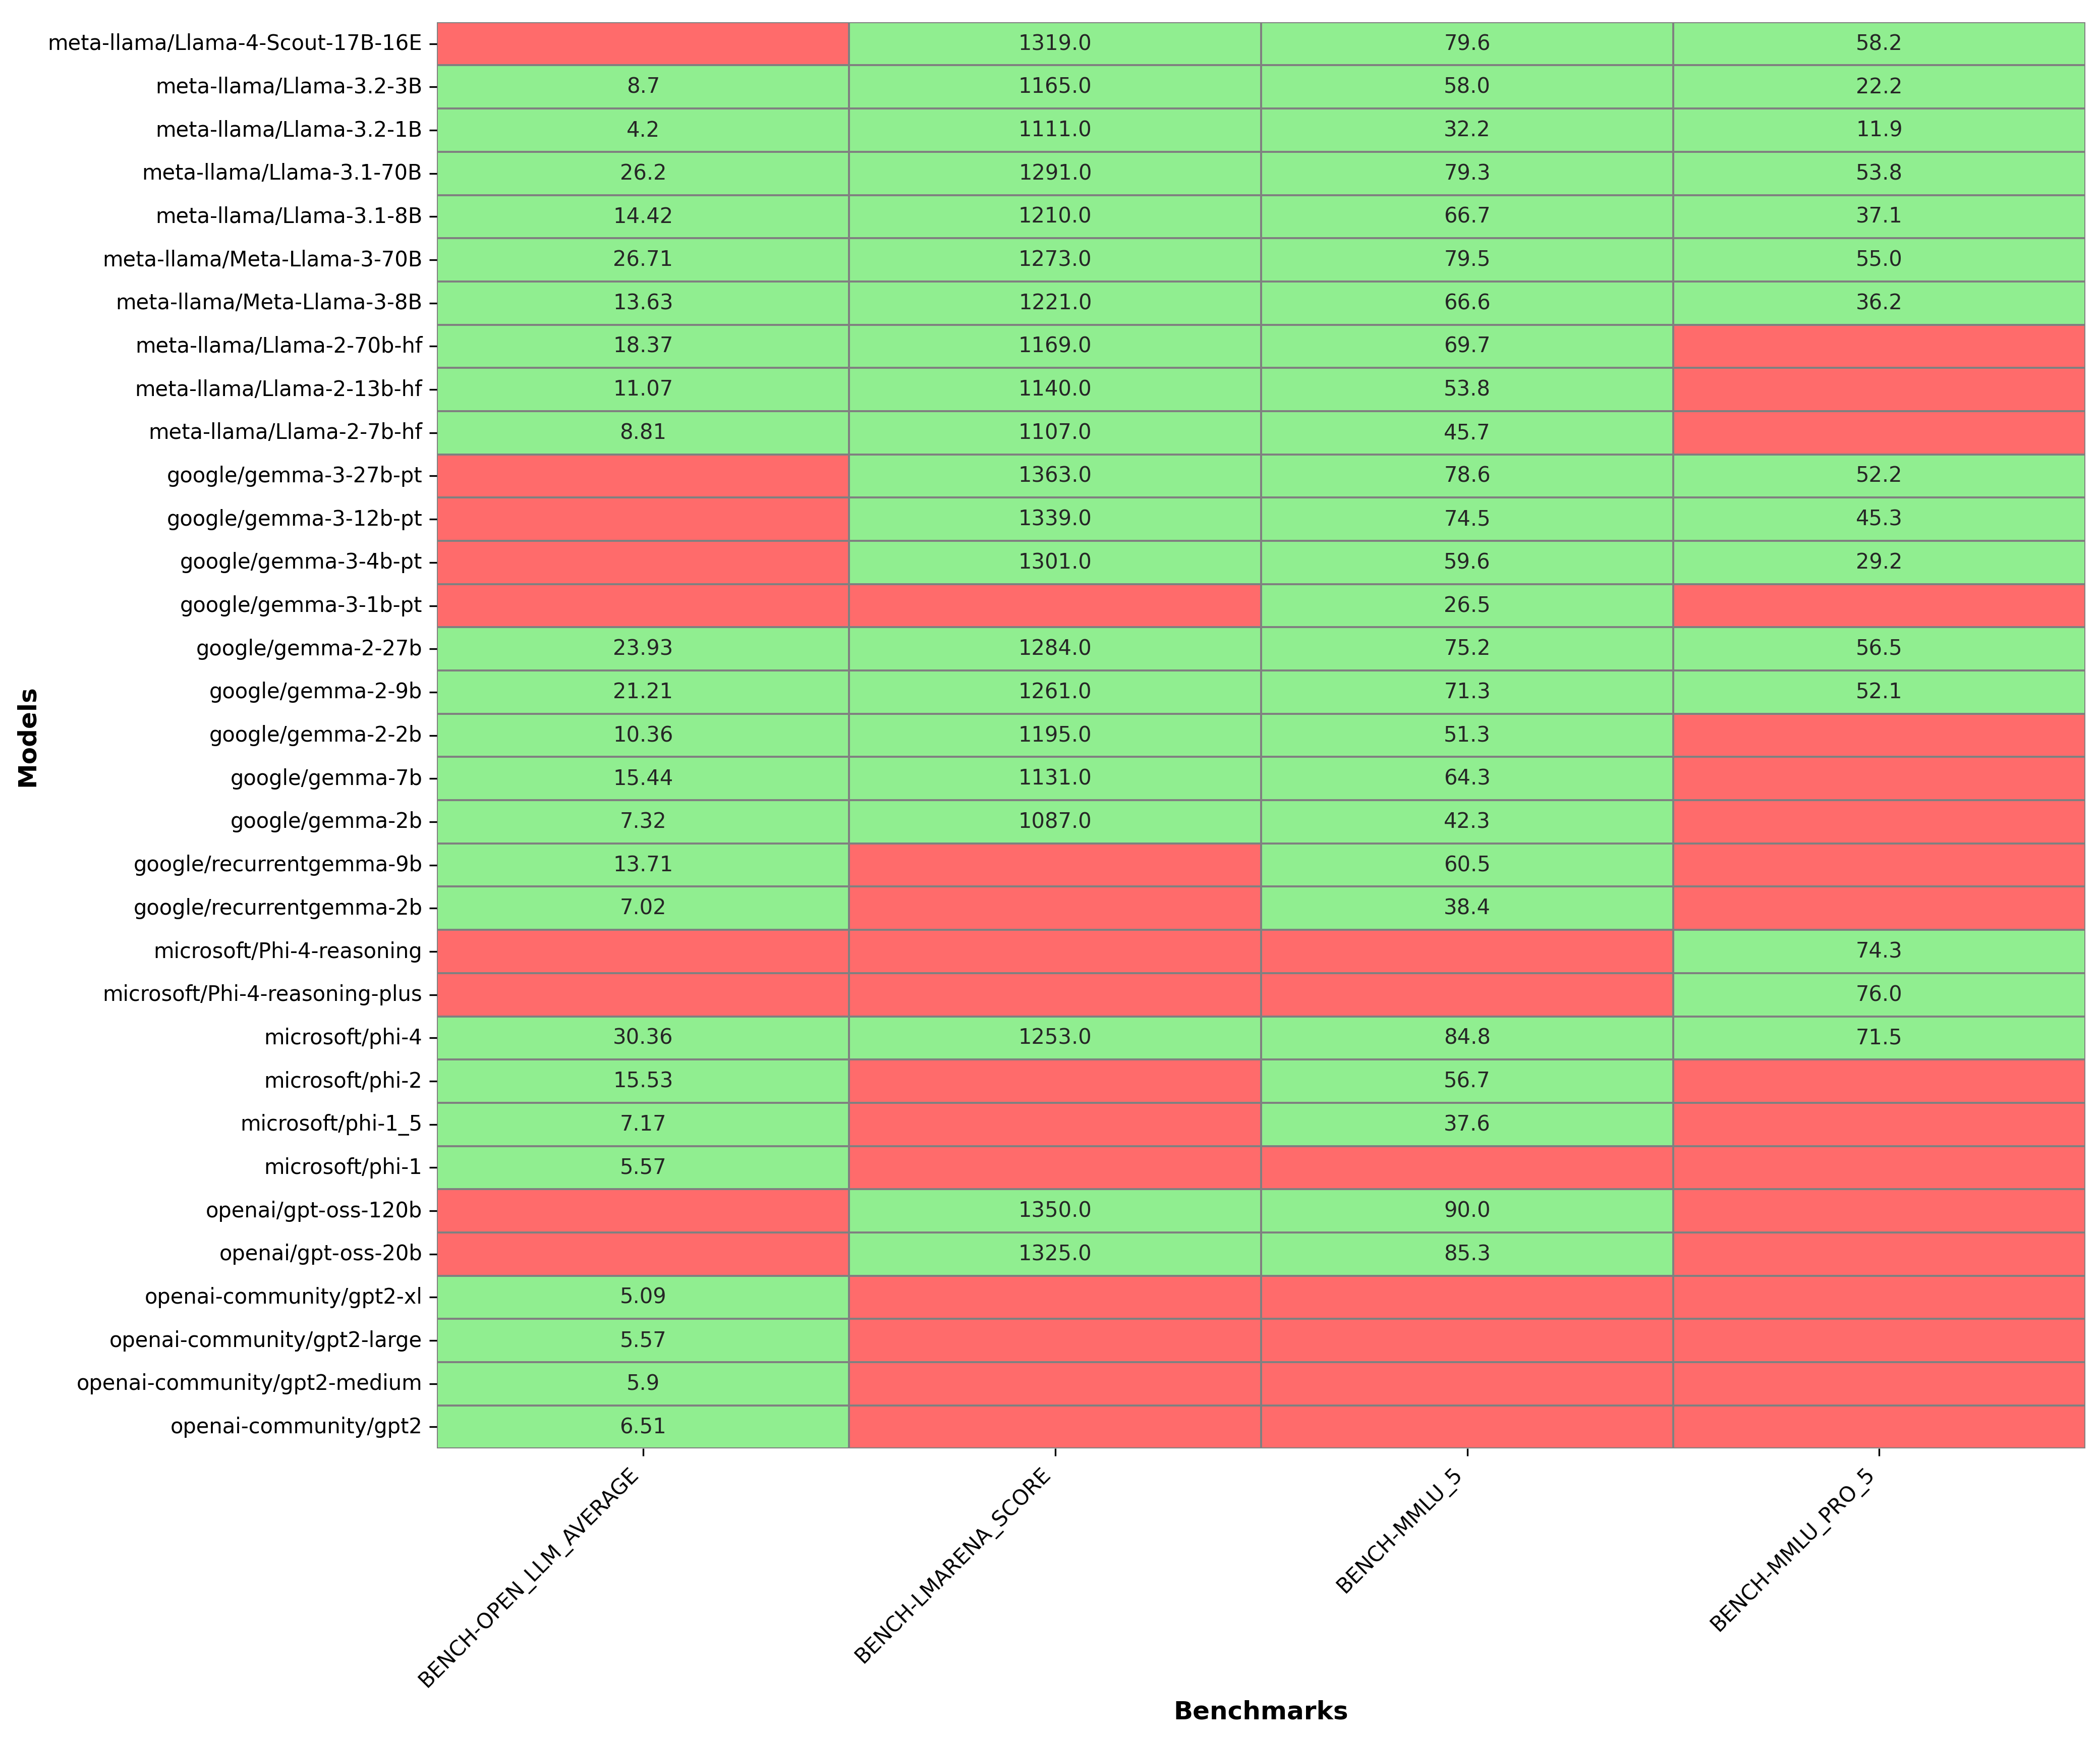
\includegraphics[width=\linewidth]{img/benchmark_availability.png}
            \caption{Availability of benchmark results for the selected models.}
            \label{fig:benchmark_availability}
        \end{figure}

\subsection{Comparing LMC Complexity and Inference Capability}




    \newpage
    \bibliography{refs}

\end{document}